\documentclass[a4paper,12pt]{article}
\usepackage{bbding,combelow,textcomp,amsfonts,amsthm,amsmath,amssymb,graphicx,color,hyperref,etoolbox}
\usepackage[utf8x]{inputenc}
\usepackage[lined,boxed,commentsnumbered]{algorithm2e}
\usepackage{tikz}

\usepackage{xeCJK}
\setCJKmainfont{PingFang TC}

\usepackage{pdfpages}

\newtoggle{story}


%%%%%%%%%%%%%%%%%%%%%%%%%%%%%%%%%%%%%%%%%%
%% Customisation options --- update as necessary
%%%%%%%%%%%%%%%%%%%%%%%%%%%%%%%%%%%%%%%%%%

%% Course details: title, semester, instructors

\newcommand{\courseTitle}{Combinatorics I (Math 7701)}
\newcommand{\semester}{Fall 2025}
\newcommand{\instructorA}{Shagnik Das}
\newcommand{\instructorB}{TA: Lu Yun-Chi}

%% Sheet number

\newcommand{\sheetNumber}{6}


%% Submission details

\newcommand{\dueDate}{15:30, Dec 9th, to be submitted on COOL.}
\newcommand{\lateWarning}{}


%% Display irrelevant footnotes?  \toggletrue for yes, \togglefalse for no

\toggletrue{story}

%%%%%%%%%%%%%%%%%%%%%%%%%%%%%%%%%%%%%%%%%%
%% End of customisation options
%%%%%%%%%%%%%%%%%%%%%%%%%%%%%%%%%%%%%%%%%%

\pdfpagewidth 8.5in
\pdfpageheight 11in
\topmargin -1in
\headheight 0in
\headsep 0in
\textheight 8.5in
\textwidth 6.5in
\oddsidemargin 0in
\evensidemargin 0in
\headheight 77pt
\headsep 0in
\footskip .75in

\makeatletter
\newcommand{\buildtitle}[4]{
\begin{flushleft}
{\large
#1
\hfill{}
#2
\par
#3
}
\end{flushleft}
\vskip 4pt
\begin{center}
{\large\bfseries#4\par}
\end{center}
\bigskip
}
\makeatother

\renewcommand{\thesection}{\normalsize\arabic{section}}

\renewcommand{\deg}{\textrm{deg}}
\newcommand{\eps}{\varepsilon}
\newcommand{\ceil}[1]{\left \lceil #1 \right \rceil}

\newcommand{\hint}{\begin{flushright} [Hint at \url{\hintURL}.] \end{flushright}}

\newcommand{\card}[1]{\left| #1 \right|}
\newcommand{\mb}[1]{\mathbb{#1}}
\newcommand{\mc}[1]{\mathcal{#1}}


\newcommand{\story}[1]{\iftoggle{story}{\footnote{#1}}{}}
\newcommand{\storymark}[1][42]{\iftoggle{story}{\footnotemark[#1]}{}}
\newcommand{\storytext}[2][42]{\iftoggle{story}{\footnotetext[#1]{#2}}{}}

\newcommand{\bonus}[2]{\paragraph{Bonus (#1 pt\ifstrequal{#1}{1}{}{s})} #2}


\begin{document}


\buildtitle{\courseTitle{}}{\semester}{\instructorA{} \hfill \instructorB{}}{Exercise Sheet \sheetNumber{}}

\vspace{-0.2in}

\begin{center}

{\bf Due date: \dueDate{}}

\end{center}

\noindent Working with your partner, you should try to solve all of the exercises below. You should then submit solutions to four of the problems, with each of you writing two, clearly indicating the author of each solution. Note that each problem is worth $10$ points, and starred exercises represent problems that may be a little tougher, should you wish to challenge yourself. In case you have difficulties submitting on COOL, please send your solutions by e-mail.

\paragraph{Exercise 1}  Recall that the Euler totient function $\phi(n)$ counts the numbers in $[n]$ that are relatively prime to $n$. Prove that $n = \sum_{d | n} \phi(d)$, where the sum is over all $d \in \mathbb{N}$ that divide $n$.

\paragraph{Solution:} (張沂魁) We first claim that for a finite poset \((P, \le)\) and \(P \subseteq \mathbb{R} \), and real functions \(f, g: P \to \mathbb{R} \), we have 
\[
	g(y) = \sum_{x \le y} f(x) \quad \forall y \in P \iff f(y) = \sum_{x \le y} g(x) \mu (x, y) \quad \forall y \in P,  
\] 
where \(\mu \) is the mobius function, the inverse function of Zeta function. We first prove from left to right. Suppose \(P = \left\{ a_i \right\}_{i=1}^n \), and without lose of generality we can extend \(\le\) to \(<\) so that \(a_1 < a_2 < \dots < a_n\). Note that if \(a_i \le a_j \) but \(a_i \neq a_j\), then \(a_i < a_j\). We define 
\[
	G = \begin{pmatrix}
		 g(a_1) \\
		 \vdots \\
		 g(a_n) \\
	\end{pmatrix}, \quad Z = \left( \zeta (a_i, a_j) \right)_{n \times n} \in M_n(\mathbb{R}), \text{ and } F = \begin{pmatrix}
		 f(a_1) \\
		 \vdots \\
		 f(a_n) \\
	\end{pmatrix},  
\]
and for every \(y \in P\), then since we know 
\[
	g(y) = \sum_{x \le y} f(x) = \sum_{i=1}^n \zeta (a_i, y) f(a_i),
\]
so we have 
\[
	G = Z^t F.
\]
Note that 
\[
	Z = \begin{pmatrix}
		1 &  &  & *  \\
		 & 1 &  &   \\
		 &  & \ddots &   \\
		0 &  &  & 1  \\
	\end{pmatrix},
\] i.e. \(Z\) is upper triangular, so \(Z^t\) is lower triangular and thus invertible since \(\det \left( Z^t \right) = 1 \) (the product of the diagonal entries). Thus, 
\[
	F = \left( Z^t \right)^{-1} G. 
\] 
Note that \(\zeta * \mu = \delta \), and converting this to the matrix representation we have 
\[
	Z \cdot M_{\mu } = I \implies M_{\mu }^t \cdot Z^t = I.
\] 
Hence, we know \(\left( Z^t \right)^{-1} = M_{\mu }^t \) since the inverse of a matrix is unique. Thus, 
\[
	F = M_{\mu }^t G,
\] i.e. 
\[
	f(a_i) = \sum_{k=1}^n \left( M_{\mu }^t \right)_{ik} g(a_k) = \sum_{k=1}^n \mu (a_k, a_i) g(a_k) = \sum_{k \le i} \mu (a_k, a_i) g(a_k).  
\]
Now since this proof is invertible, so we know the if and only if statement holds. Now suppose \((P, \le) = ([n], \cdot \mid \cdot)\), which is the division poset of \([n]\), where \(n\) is a fixed positive integer. Hence, we know 
\[
	g(y) = \sum_{x | y} f(x) \quad \forall y \in [n] \iff f(y) = \sum_{x \mid y} g(x) \mu (x, y) \quad \forall y \in [n].  
\]   
Note that for every fixed \(x\), the construction of \(\mu \) is 
\[
	\mu (x, x) = 1, \quad \mu (x, y) = - \sum_{x \mid z \mid y, x \neq z} \mu (z, y) \text{ for } x \mid y, x \neq y. 
\]  
Equivalently, we have 
\[
	\sum_{x \mid z \mid y} \mu (z, y) = 0. 
\]
Thus, for every \(x \mid y\), we have \(\mu (x,y) = \mu \left( 1, \frac{y}{x} \right) \). From now on, we refer \(\mu (1, n)\) to \(\mu (n)\). Thus, we have
\[
	\sum_{d \mid n} \mu (d) = 0, \quad \mu (1) = 1. 
\]      
Hence, for prime \(n\), we know 
\[
	\mu (1) + \mu (n) = 0 \implies \mu (n) = -1.
\] 
\paragraph{Claim:} \(\mu \left( p^k \right) = 0 \) for \(k \ge 2\) and any prime \(p\).  
\paragraph{Proof:} For \(k = 2\), since 
\[
	\mu (1) + \mu (p) + \mu \left( p^2 \right) = 0, 
\]   
and since \(\mu (p) = -1\), so we're done. Now suppose for \(k \le \ell \) this is true, then since 
\[
	0 = \sum_{d \mid p^{\ell + 1}} \mu (d) = \mu (1) + \mu (p) + \dots + \mu (p^{\ell } ) + \mu \left( p^{\ell + 1} \right) = \mu (1) + \mu (p) + \mu \left( p^{\ell + 1} \right),  
\]  
so we have \(\mu \left( p^{\ell + 1} \right) = 0 \), and we're done. 
\paragraph{Claim:} If \(\gcd(a, b) = 1\), then \(\mu (ab) = \mu (a) \mu (b)\). 
\paragraph{proof:} We prove it by induction on \(ab\). For \(ab = 1\), then \(a = 1, b = 1\), and since 
\[
	1 = \mu (1) = \mu (1 \cdot 1) = \mu (1)^2,
\]  
so the base case is true. Now suppose for all \(ab \le k\) this is true. Then, for all \(a^{\prime} b^{\prime} = k + 1\) and \(\gcd \left( a^{\prime} , b^{\prime}  \right) = 1 \) , we have 
\begin{align*}
	\mu \left( a^{\prime} b^{\prime}  \right) &= -\sum_{\substack{d \mid a^{\prime} b^{\prime} \\ d \neq a^{\prime} b^{\prime} }} \mu (d) = - \sum_{\substack{e \mid a^{\prime}  \\ f \mid b^{\prime}  \\ ef \neq a^{\prime} b^{\prime} }} \mu (ef)  = -  \sum_{\substack{e \mid a^{\prime}  \\ f \mid b^{\prime}  \\ ef \neq a^{\prime} b^{\prime} }} \mu (e) \mu (f) \\
	&= - \sum_{e \mid a^{\prime} } \mu (e) \sum_{\substack{f \mid b^{\prime}  \\ ef \neq a^{\prime} b^{\prime} }} \mu (f) = - \left( \sum_{e \mid a^{\prime} } \mu (e) \sum_{f \mid b^{\prime} } \mu (f) - \mu (a^{\prime} ) \mu (b^{\prime} )   \right) \\
	&= - \left( \sum_{ef \mid a^{\prime} b^{\prime} } \mu (e) \mu (f) - \mu (a^{\prime} ) \mu (b^{\prime} )  \right) = - \left( \sum_{ef \mid a^{\prime} b^{\prime} } \mu (ef) - \mu (a^{\prime} ) \mu (b^{\prime} )  \right) \\ &= -(-\mu (a^{\prime} ) \mu (b^{\prime} )) = \mu (a^{\prime} ) \mu (b^{\prime} ).   
\end{align*}
Hence, we can conclude that 
\[
	\mu (n) = \begin{cases}
		1, &\text{ if } n = 1 ;\\
		(-1)^k, &\text{ if } n = p_1 p_2 \dots p_k \text{ where } p_{i} \text{'s} \text{ are prime}   ;\\
		0, &\text{ otherwise} .
	\end{cases}
\]
For \(n = 1\), it is trivial. As for \(n = p_1 p_2 \dots p_k\) where \(p_i\)'s are all prime, since we know 
\[
	\mu (n) = \mu (p_1) \mu (p_2) \dots \mu (p_k) = (-1)^k,
\]   
so this is true. For the "otherwise" case, since we know \(p^2 \mid n\) for some prime \(p\) and 
\[
	\mu (n) = \mu \left( p^2 \right) \mu \left( \frac{n}{p^2} \right) = 0 \cdot \mu \left( \frac{n}{p^2} \right) = 0,   
\]  
so this is also true. By this, we know 

\[
	g(y) = \sum_{x | y} f(x) \quad \forall y \in [n] \iff f(y) = \sum_{x \mid y} g(x) \mu \left( \frac{y}{x} \right)  \quad \forall y \in [n],
\]
and now we know the value of \(\mu \left( \frac{y}{x} \right) \). 

Now we can start to prove the problem. Suppose \(s = p_1^{\alpha _1} p_2^{\alpha _2} \dots p_k^{\alpha _k}\), where \(p_i\)'s are prime, then we know 
\begin{align*}
	\phi (s) &= s \left( 1 - \frac{1}{p_1} \right) \left( 1 - \frac{1}{p_2} \right) \dots \left( 1 - \frac{1}{p_k} \right) \\
	&= s \left( \sum_{I \subseteq [k]} \prod _{i \in I} \left( -\frac{1}{p_i} \right)   \right) = s \sum_{I \subseteq [k]} (-1)^{\vert I \vert } \frac{1}{\prod _{i \in I} p_i} = s \sum_{d \mid s} \frac{\mu (d)}{d} \\
	&= \sum_{d \mid s} \frac{s}{d} \mu (d) = \sum_{e \mid s} e \mu \left( \frac{s}{e} \right).        
\end{align*}  
Note that we let \(e = \frac{s}{d}\) in the last step, and this statement is true for all \(s \in [n]\). Now if we let \(\phi = f\) and \(g(x) = x\), then we know 
\[
	g(y) = \sum_{x \mid y} f(x) \implies y = \sum_{x \mid y} \phi (x).  
\]  
In particular, we can choose \(y = n\) so that 
\[
	n = \sum_{x \mid n} \phi (x), 
\] 
and since this proof is true for all \(n\), so we can conclude that 
\[
	n = \sum_{d \mid n} \phi (d) \text{ for all } n \in \mathbb{N}.  
\] 



\paragraph{Exercise 2}  Recall that a chain $C$ in a poset $(P, \le)$ is a subset $C \subseteq P$ where every pair of elements $x, y \in C$ is comparable.  Consider the infinite poset $(2^{\mathbb{N}}, \subseteq)$, where the elements are (possibly infinite) subsets of $\mathbb{N}$, ordered by inclusion.
\begin{itemize}
	\item[(a)] Show that this poset has a countably infinite\footnote{A set $S$ is countably infinite if there is a bijection from $S$ to $\mathbb{N}$.  In other words, you can list the elements $S = \{ s_1, s_2, s_3, s_4, \hdots \}$, with every element of $S$ appearing within some finite number of terms.} chain.
	\item[(b)*] Is there an uncountable\footnote{A set is uncountable if it is infinite, but not countably so.  That is, there is no injection from $S$ into $\mathbb{N}$.} chain in the poset?
\end{itemize}
\paragraph{Solution:} (張沂魁) 
\begin{itemize}
	\item [(a)] Consider 
	\[
		a_1 = \left\{ 1 \right\}, a_{n + 1} = a_n \cup \left\{ n + 1 \right\} \text{ for all } n \ge 1,    
	\]
	so we know \(C_1 = \left\{ a_i \right\}_{i=1}^{\infty}  \) is an infinite chain. Note that \(C_1\) is countable since we can make a bijeciton from \(C_1\) to \(\mathbb{N} \) by \(f\), where 
	\[
		f(a_i) = i \text{ for all } i \in \mathbb{N}. 
	\]     
	\item [(b)] Since \(\mathbb{Q} \) is countable, so we can enumerates \(\mathbb{Q} \) as \(\left( q_n \right)_{n=1}^{\infty}  \). Now consider 
	\[
		S_x = \left\{ n \in \mathbb{N} : q_n < x \right\} \quad \forall x \in \mathbb{R},
	\]
	then we know 
	\[
		C_2 = \left\{ S_x : x \in \mathbb{R}  \right\} 
	\]
	is an infinite chain since for all \(a, b \in C_2\), we know \(a = S_x\) and \(b = S_y\) for some \(x, y \in \mathbb{R} \), and WLOG suppose \(x \le y\), then \(S_x \subseteq S_y\) since \(w \in S_x\) iff \(q_w < x\), and this gives \(q_w < x \le y\), and thus \(w \in S_y\). Hence, \(a = S_x \subseteq S_y = b\). Note that there is a bijection \(g\) between \(C_2\) and \(\mathbb{R} \) by 
	\[
		g \left( S_x \right) = x \in \mathbb{R}, 
	\]          
	and since \(\mathbb{R} \) is uncountable, so \(C_2\) is also uncountable, and we're done.  
\end{itemize}

\paragraph{Exercise 3}
Let $n \ge 1$ be odd. For a family $\mathcal F \subseteq \binom{[n]}{k}$ of subsets of size $k$ of a ground set $[n]$, we define its \emph{shadow} $\partial \mathcal F = \{ G \in \binom{[n]}{k-1} : \exists F \in \mathcal F \textrm{ such that } G \subset F \}$ to be the $(k-1)$-sets that are contained in some set of $\mathcal F$.
\begin{itemize}
	\item[(a)] Show that for every $\mathcal{F} \subseteq \binom{[n]}{\frac{n+1}{2}}$, we have $|\partial \mathcal F| \ge |\mathcal F|$.
	\item[(b)] Prove that if $\mathcal{A} \subseteq 2^{[n]}$ is an antichain of size $\binom{n}{\frac{n+1}{2}}$ with $\mathcal A \notin \{ \binom{[n]}{\frac{n-1}{2}}, \binom{[n]}{\frac{n+1}{2}} \}$, then there must be some non-empty $\mathcal F \subsetneq \binom{[n]}{\frac{n+1}{2}}$ with $|\partial \mathcal F | = |\mathcal{F}|$.
	\item[(c)] Deduce that the only maximum antichains in $2^{[n]}$ are $\binom{[n]}{\frac{n-1}{2}}$ and $\binom{[n]}{\frac{n+1}{2}}$.
\end{itemize}

\paragraph{Exercise 4}  Let $\mathcal{B}_n = \left( 2^{[n]}, \subseteq \right)$ be the Boolean poset of all subsets of $[n]$, ordered by inclusion. A symmetric chain in $\mathcal{B}_n$ is a chain $S_k \subseteq S_{k+1} \subseteq \hdots \subseteq S_{n-k}$ such that $|S_i| = i$ for all $i$. Prove that for all $n \ge 1$, $\mathcal{B}_n$ can be partitioned into symmetric chains.
\paragraph{Solution:} (黃子恆) See last few pages.

\paragraph{Exercise 5}  A family $\mathcal F = \{ F_1, F_2, \hdots, F_m \}$ of subsets of $[n]$ is said to be \emph{separating} if for any two elements $1 \le i < j \le n$, there is some set $F \in \mathcal F$ such that $\card{F \cap \{i,j\}} = 1$; that is, the set $F$ differentiates between $i$ and $j$.
\begin{itemize}
	\item[(a)] Prove that the smallest separating family has size $\ceil{\log_2 n}$.
\end{itemize}
The family is said to be \emph{strongly separating} if even more is true: for every $1 \le i < j \le n$, there are sets $F, G \in \mathcal F$ such that $F \cap \{i,j\} = \{i\}$ and $G \cap \{i,j\} = \{j\}$.
\begin{itemize}
	\item[(b)] Prove that the smallest strongly separating family has size $m$, where $m$ is the smallest natural number satisfying $\binom{m}{\ceil{m/2}} \ge n$.\footnote{When $n$ is large, we have $m = \log_2 n + \frac12 \log_2 \log_2 n + O(1)$.}
\end{itemize}

\paragraph{Exercise 6}  Consider the poset $(P, \le)$ whose Hasse diagram is given in Figure 1.
\begin{itemize}
	\item[(a)] For every pair $i,j \in [6]$, determine value of the M\"obius function $\mu (i,j)$.
	\item[(b)] Prove that for any finite poset $(P,\le)$ and all $x,y \in P$, $\mu(x,y)$ is always an integer.
\end{itemize}
\begin{figure}[h]

\centering

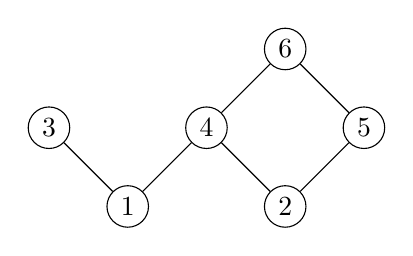
\begin{tikzpicture}
  [scale=1.0,auto=left,every node/.style={circle, draw, color=black!100, inner sep=0pt, minimum width=15pt}]

 \node (n1) at (1,0) {$1$};
 \node (n2) at (3,0) {$2$};
 \node (n3) at (0,1) {$3$};
 \node (n4) at (2,1) {$4$};
 \node (n5) at (4,1) {$5$};
 \node (n6) at (3,2) {$6$};

 \foreach \from/\to in {n1/n3, n1/n4, n2/n4, n2/n5, n4/n6, n5/n6}
   \draw (\from) -- (\to);

\end{tikzpicture}
\caption{The Hasse diagram of a poset.}
\end{figure}
\paragraph{Solution:} (黃子恆) See last few pages.

\includepdf[pages=-]{./HW6Conc.pdf}

\end{document}